\chapter{Requirements and design} \label{chap:reqs}

The following section presents the identified objectives and the methodology we follow for the implementation of $MQuicTT$.
We discuss the steps we have taken to analyse the existing QUIC and MQTT implementations to motivate our choice of libraries.
Additionally, we describe the design choices taken.

\section{Requirements}

QUIC theoretically presents benefits in terms of faster connection times and resilience to packet loss.
IoT devices that save energy by turning themselves off or disconnecting from the network when they are unused can benefit from faster reconnection times.
Additionally, higher resilience to packet loss can be beneficial for IoT deployments where many devices on data links may cause congestion.
However, due to the introduction of streams and other features that provide these performance guarantees, QUIC is also a relatively complex protocol.
Hence, we must analyse if this complexity translates into challenges for hardware constrained devices.

As previously discussed, IoT devices often carry sensitive data; hence, we must also consider that communication should be safe and secure.
This requirement leads us to two choices.
Firstly, we only consider communication that happens over an encrypted channel, that is, a network connection secured by TLS.
This also gives us a chance to test QUIC's claim of faster secure connections due to a less complex handshake.
Secondly, we must consider the programming language that we use for the implementation.
Modern systems programming is dominated by C; however, the weak type system of C leads to many vulnerabilities stemming from bad memory management and race conditions.
This means that insecure firmware may be shipped from the manufacturer and deployed when an IoT system is installed.
The issue of such bugs in systems languages has led to the creation of the Rust programming language, which uses an ownership memory management system to mitigate these bugs.
However, Rust is a relatively new programming language and does not yet benefit from the years of optimisations and ecosystem support that C has.
Rust also opts to use a dependency manager that packages external dependencies into the binary of the program, which may have an effect on the binary size of the implementation.
Hence, it is still important to contrast Rust with other languages.

We focus on the MQTT protocol as it is the most popular application layer protocol in the IoT space~\citep{tmobile_iot}.
MQTT is also beneficial for the analysis due to it being lightweight and having a low code footprint.
This means that the implementation of MQTT itself should not be a bottleneck for hardware constrained devices.
Hence, with the high-level goal of analysing the viability of a safe implementation of QUIC as a transport layer protocol for IoT devices, we must create an implementation that can be used as a test bench for such an analysis.
This implementation will be a QUIC-based implementation of the MQTT protocol in a safe programming language.

We must then analyse the resulting implementation in terms of network performance and the constraints of IoT devices.
For network performance, we must evaluate if the QUIC-based implementation is at least as performant as its TCP counterpart.
In terms of hardware constraints, we have chosen to focus on the storage constrained in IoT devices.
We focus specifically on storage as we predict that this is where our implementation will see the biggest challenge.
The requirements of using TLS, as well as the relatively untested binary sizes produced by Rust, mean that the implementation could be too large to act as firmware for devices with extreme hardware constraints.

Hence, from these high-level requirements, to analyse QUIC as a transport layer protocol for IoT, we have identified the following specific requirements using a MoSCoW style analysis:

\begin{itemize}
    \item Must:
    \begin{itemize}
        \item We \textbf{must} create a test case for MQTT using QUIC - MQuicTT.
        \item We \textbf{must} analyse the performance of MQuicTT compared to base MQTT implementations.
        \item We \textbf{must} focus on realistic testing scenarios for evaluation.
    \end{itemize}
    \item Should:
    \begin{itemize}
        \item We \textbf{should} analyse a general methodology for reducing the hardware footprint of transport layer protocols for IoT.
        \item We \textbf{should} analyse the hardware footprint and feature set of the chosen QUIC and TLS libraries.
    \end{itemize}
    \item Could:
    \begin{itemize}
        \item We \textbf{could} create a QUIC extension that uses a lightweight security protocol.
    \end{itemize}
\end{itemize}

The creation of $MQuicTT$ is not only important to be able to evaluate the usage of QUIC for IoT, but also to test the viability of porting an MQTT implementation to QUIC in Rust.

We treat the base version of MQTT as the standard for comparisons as this will be an industry used TCP implementation of the protocol.
A comparison to this will be made in terms of network performance and storage use.
We have chosen to focus on the storage constraint of IoT hardware as this is often the hardest requirement to fulfil.
Storage also often dictates the other hardware specifications for the device as it usually takes up most physical space.

As previously discussed, we analyse the viability of creating a general methodology for reducing the QUIC stack for IoT devices following the methodology of~\cite{eggert_towards_2020}.
To do this, we must also analyse the storage footprint of each feature of the transport layer stack.
By features, we mean the features as described in the protocol's respective RFC.
For QUIC, for example, this could be the 0-RTT or connection migration features.
If any of these are heavy in terms of required storage space and not necessary for IoT devices, we could extract them from the implementation.

Finally, we hypothesise that TLS takes a lot of storage space and hardware, again, based on the analysis performed by~\cite{eggert_towards_2020}.
Hence, it could be possible to create a QUIC extension with a lightweight security protocol such as KP-ABE.
Such an extension, however, may be out of the scope of this work.

From these requirements, we have split the project into the following objectives:

\begin{itemize}
    \item \textbf{O1}: Compare existing QUIC and MQTT implementations that can act as underlying libraries.
    \item \textbf{O2}: Create an abstraction layer for the QUIC specific logic.
    \item \textbf{O3}: Implement MQuicTT by changing the underlying MQTT implementation to use this abstraction layer.
    \item \textbf{O4}: Create a test bench for the network performance analysis of MQuicTT.
    \item \textbf{O5}: Devise a methodology for trimming down the QUIC stack in terms of binary size.
    \item \textbf{O6}: Analyse the components of the MQuicTT binary.
\end{itemize}

\textbf{O1} focuses on finding implementations that can be used as the underlying libraries for $MQuicTT$.
As discussed in Section~\ref{sec:mquictt_design}, we have opted to use existing implementations; hence we must compare them based on our criteria of performant, safe implementations that fit IoT storage constraints.

We have also opted to create an intermediate layer to encapsulate the QUIC protocol logic in the implementation.
Hence, \textbf{O2} focuses on creating this abstraction.

\textbf{O3} describes the core of the implementation of $MQuicTT$.
Using the libraries identified in \textbf{O1} and the abstraction created in \textbf{O2} we must create a port of the chosen MQTT implementation using QUIC.

We then move to the evaluation stage of the project; hence, creating a test bench in \textbf{O4} will be crucial for the network performance portion of this evaluation.

In \textbf{O5} we then focus on the storage analysis of the resulting implementation and devise methods for trimming down the QUIC stack.
We also analyse the components of the resulting binaries in \textbf{O6} to find where the contributions to the binary size come from exactly.

Hence, the rest of this chapter is split into sections corresponding to the design for the implementation centred objectives, that is, \textbf{O1}, \textbf{O2}, \textbf{O3}.
The rest of the objectives are addressed in Chapter~\ref{chapter:eval}.

\section{Design of the implementation}

In this section, we present a comparison of existing QUIC and MQTT implementations that can be used as underlying libraries for MQuicTT.Additionally, we discuss the high-level design of MQuicTT and the approach we have taken when it comes to using existing libraries compared to creating new protocol implementations.

\section{Overall MQuicTT design} \label{sec:mquictt_design}

We first analyse what is required to create $MQuicTT$ based on the established requirements and objectives.

We opt to use existing implementations of QUIC and MQTT.
An alternate approach to this would be creating implementations from scratch that could be optimised for our use case.
However, we demonstrate an actual use case by opting to use existing libraries.
These libraries have both been built for production use and are relatively widely deployed.
Hence, we are more likely to get accurate results.
In addition to this, the development time needed to create implementations for these protocols from scratch would far exceed this project's scope.

Secondly, we must create an intermediate library that will act as an abstraction from the QUIC logic - $QuicSocket$.
By creating this intermediate library and ensuring that its API mimics a standard TCP socket, we lower the difficulty of porting $rumqtt$ to QUIC.
Additionally, this library can be used for any application that uses the QUIC protocol.
The key consideration when creating this abstraction is how we want to use QUIC streams.

To recap, QUIC streams are an encapsulation around the data transfer portion of the QUIC protocol.
After establishing a connection, QUIC opens streams in order to send and receive data.
There can be an arbitrary number of streams on a single UDP connection using QUIC.
Hence, QUIC provides advantages by removing head-of-line blocking as different logical separations of data can be sent on different streams.
For example, we can opt to send an HTML file and a stylesheet for a website on different streams so that if a packet of the stylesheet gets lost, the HTML can still be rendered.

We can also use this strategy to improve the performance of $MQuicTT$ by choosing an appropriate encapsulation.
There are two main possibilities here.
Firstly, we may opt to send a single MQTT connection on a QUIC stream.
Secondly, we may opt to treat every subscription to a broker as a separate QUIC stream.
The specifics of our choice and a discussion on this topic can be found in Chapter~\ref{chap:impl}.

Hence, the design for the implementation has been split into the following stages.
Firstly, we must find appropriate implementations of QUIC and MQTT based on our criteria.
Although we opt to use a Rust implementation, it is still important to consider other systems-language based implementations of QUIC.
If the Rust implementations of the protocol stand out in terms of storage consumption compared to, for example, C++, this would indicate that Rust is perhaps less suitable for this application.
Secondly, we must create an abstraction around the chosen QUIC implementation that acts as a socket for the QUIC protocol.
This abstraction must have the functionality required to securely transfer data using QUIC.
That is, we must be able to work with TLS keys, establish a secure connection and send and receive data using streams.
This library must also have an API similar to that of the TCP sockets API for external consistency.
This means that we must have functions that take in buffers, write or read from those buffers, and return the number of bytes that were read or written.
Adhering to this API will also simplify the port.
Lastly, we must use the resulting socket library to port the chosen MQTT implementation to QUIC.

Further discussion of specific technical choices that we have made during the implementation can be found in Chapter~\ref{chap:impl}.

\subsection{QUIC} \label{section:quic_impl}

We now compare the existing implementations of the QUIC protocol in the context of usability for IoT devices and present the reasoning behind our choice of QUIC library.
We have considered the mainstream implementations in the C, C++, Rust and Go programming languages as these are the languages that can be considered systems languages and would thus be the most widely used ones for IoT devices.
In addition to this, we did not consider implementations paired with a browser web engine as these would be impossible to use on hardware constrained devices.
Hence, we did not include notable implementations such as the QUIC implementation of the chromium web engine~\citep{chromium_quic_2021} and $Neqo$~\citep{mozilla_neqo_2022}.

Importantly, to analyse the performance of underlying QUIC implementations, we have transferred the same file using each implementation several times and have taken the average time to do so.
We repeated this while altering parameters as described in Section~\ref{chap:net_sim}.
The differences in transfer time were negligible and have hence not been presented as part of the comparison of libraries.
Hence, we compare QUIC implementations in terms of their TLS use, programming language and the binary size produced by their client and server implementations.

First, we consider the general landscape of available QUIC implementations to contextualise the ones developed in Rust.
Table~\ref{tab:quics} demonstrates the analysed QUIC implementations.
In order to find the size of the binary, we have used the Linux $ls$ utility.
In the case of the $mvfst$ implementation, we have taken further steps due to the reported binary size being far too large.
Therefore, we had to remove the C++ debug symbols that were causing the binary size to be over 300 MiB.
We have identified the following main methods by which QUIC implementations incorporate TLS:

\begin{itemize}
    \item Use of an external library - the implementation uses an external TLS API either by using a package manager in the case of Rust or by relying on an installed implementation in the case of C and C++.
    \item Use of own implementation - the implementation packages its implementation of the TLS protocol alongside QUIC.
\end{itemize}

This different use of TLS presented a challenge in calculating the binary size of the QUIC servers and clients.

\begin{table}[ht]
    \caption{The identified QUIC implementations and their binary size footprint. The footprint has been split into a client and server footprint using a minimal reproducible example for each. We used each implementation to create an example client and server capable of sending and receiving QUIC packets and analysed the binary size. Where provided, we compared this to the given examples to ensure as little implementation bias as possible. However, this is still not a perfect estimate, and some variance due to implementation details may be present.}\label{tab:quics}
    %\tt 
    \rowcolors{2}{}{gray!3}
    \begin{tabular}{@{}lllll@{}}
        \toprule
        \textbf{Implementation} & \textbf{PL}   & \textbf{Footprint (client) (MiB)} & \textbf{Footprint (server) (MiB)} & \textbf{TLS method} \\
        ngtcp2                  & \texttt{C}    & \texttt{3.4}                      & \texttt{4.3}                      & \texttt{External}   \\
        picoquic                & \texttt{C}    & \texttt{3.2}                      & \texttt{3.9}                      & \texttt{External}   \\
        msquic                  & \texttt{C}    & \texttt{3.2}                      & \texttt{4.1}                      & \texttt{External}   \\
        quic-go                 & \texttt{Go}   & \texttt{8.7}                      & \texttt{9.9}                      & \texttt{External}   \\
        Quinn                   & \texttt{Rust} & \texttt{9.1}                      & \texttt{9.5}                      & \texttt{External}   \\
        Quiche                  & \texttt{Rust} & \texttt{7.8}                      & \texttt{7.0}                      & \texttt{Own}        \\
        mvfst                   & \texttt{C++}  & \texttt{11.1}                     & \texttt{12.0}                     & \texttt{Own}        \\
        \bottomrule
    \end{tabular}
\end{table}

Specifically, in each case, we have considered the external dependencies that a developer will have to install to run the QUIC implementation on a device.
Hence, in the case of C implementations that require an external TLS library, such as OpenSSL, to be installed and linked on the system, we have opted to add the binary size produced by OpenSSL to the size of the QUIC binaries.
Additionally, in the case of $picoquic$, we have added the size of the $picotls$ dependency on top of the size of OpenSSL.

\begin{figure}[ht]
    \centering
    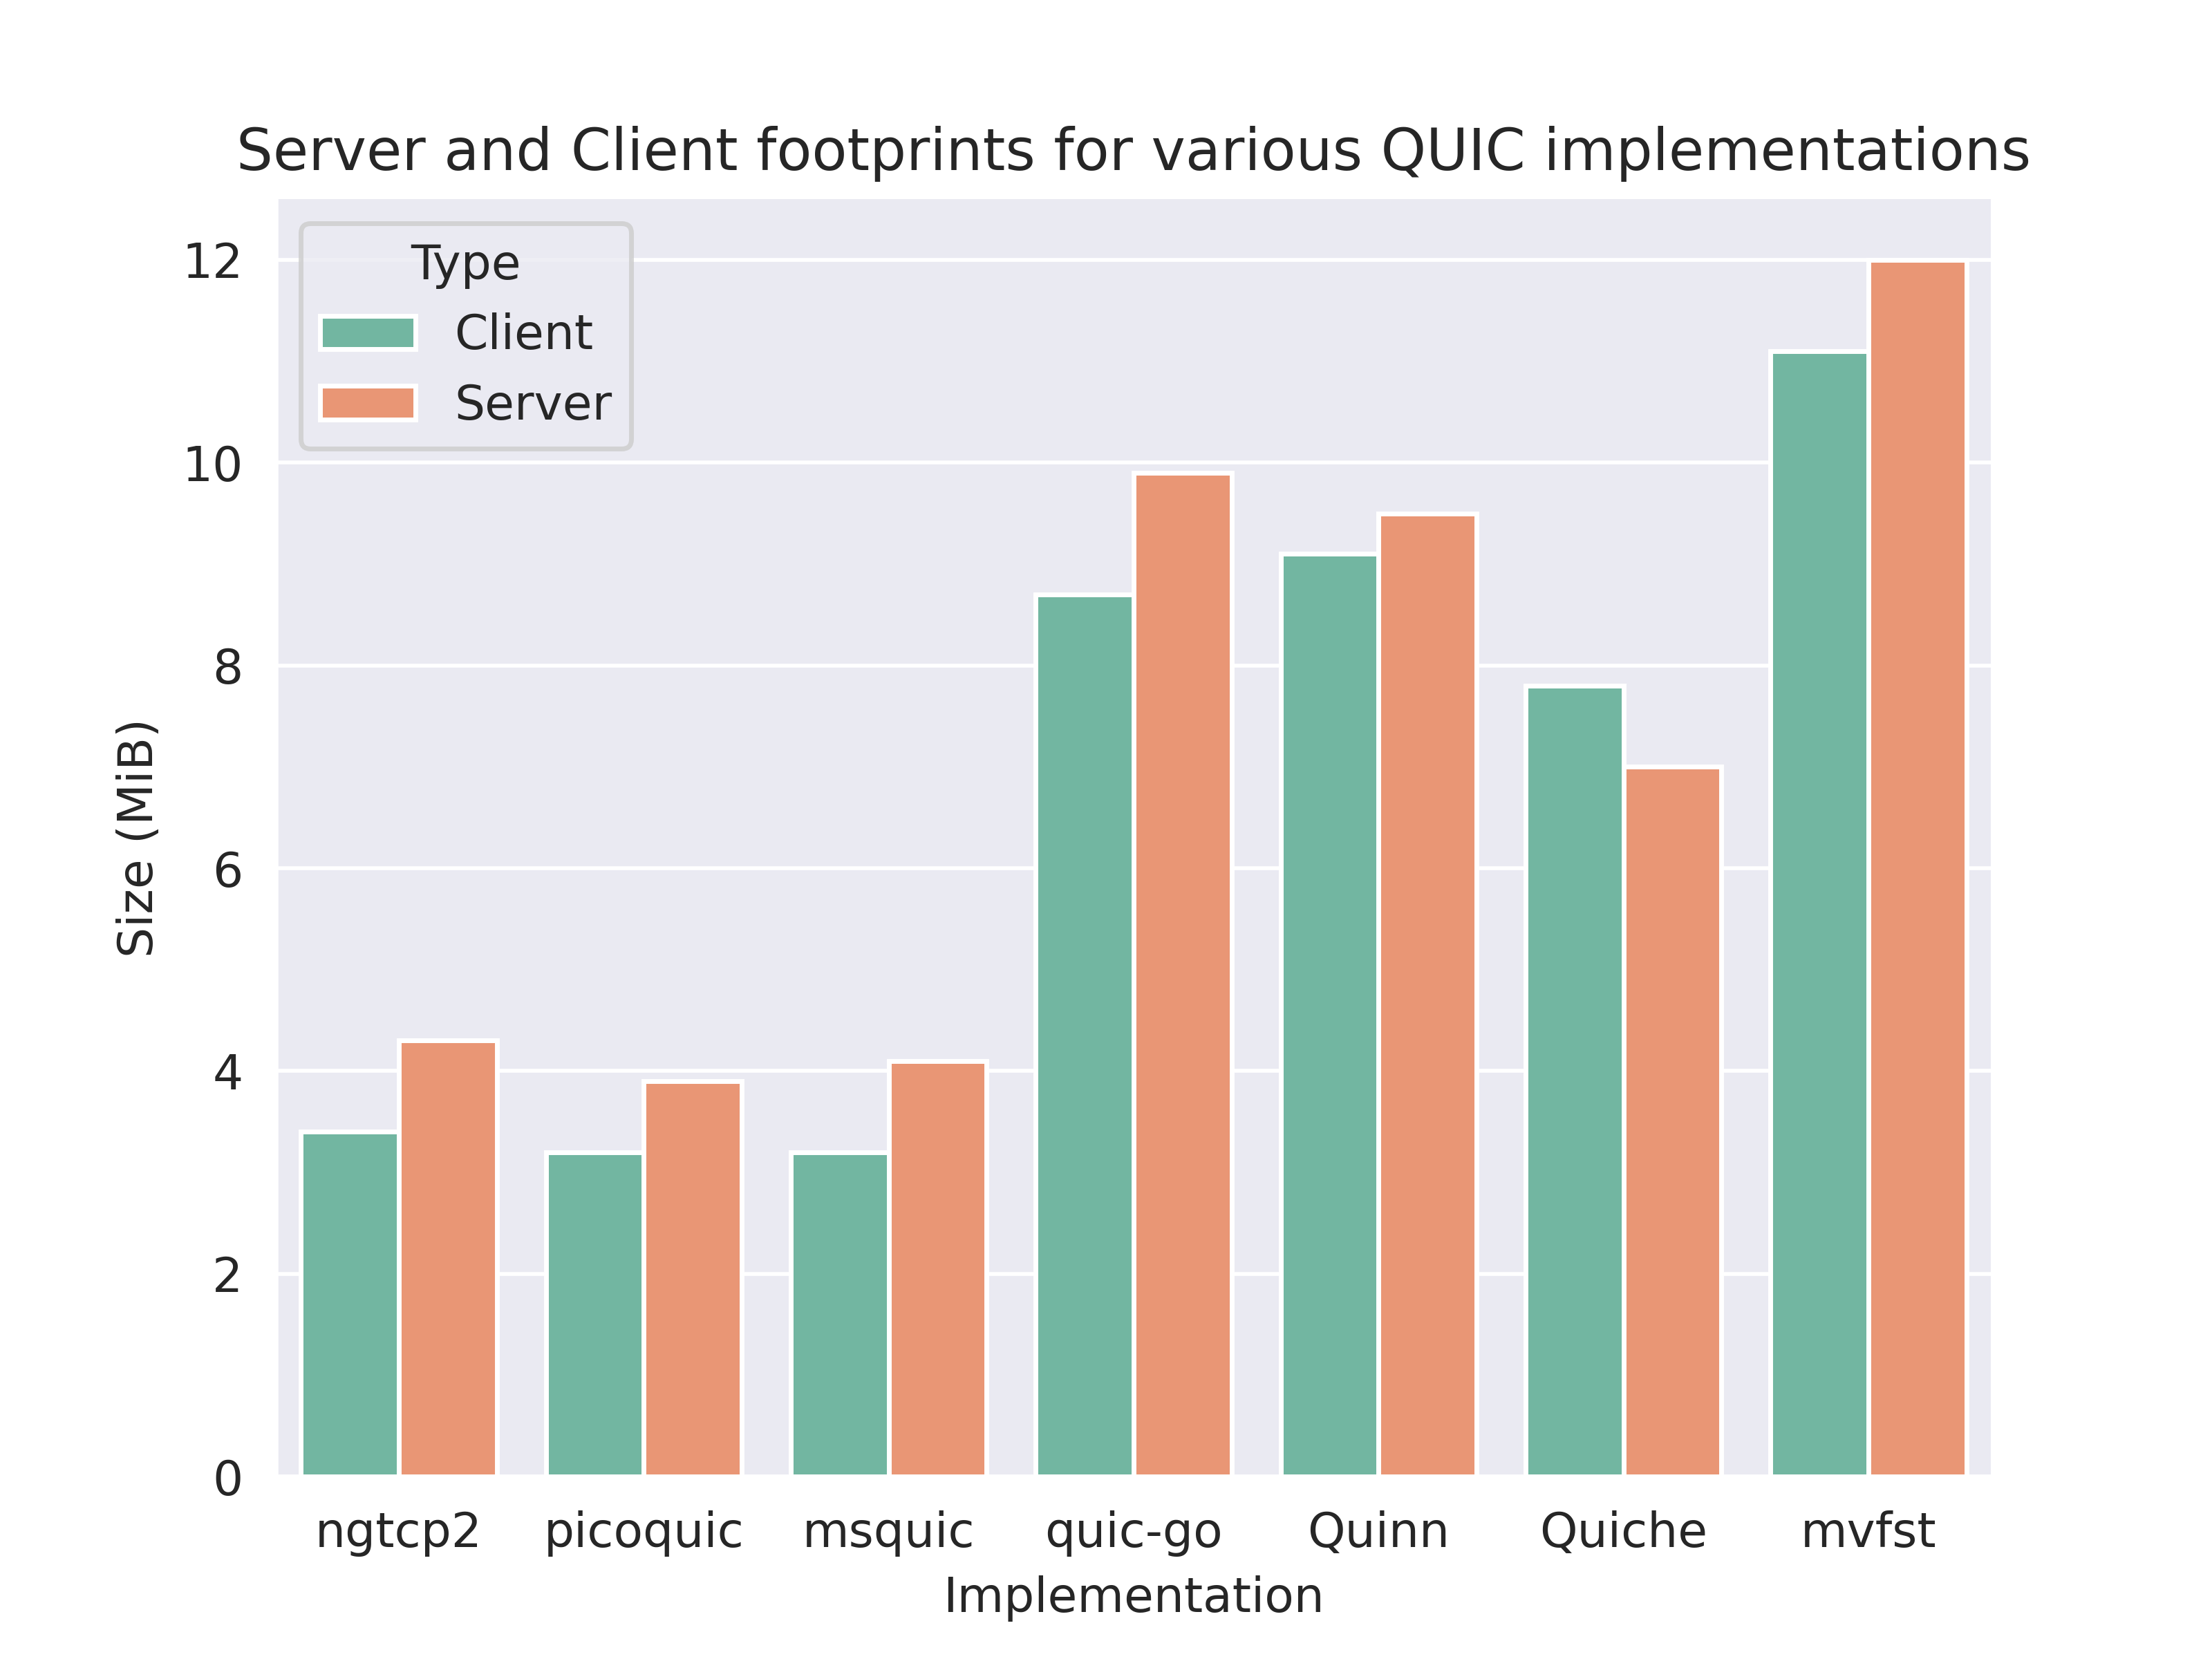
\includegraphics[width=1\linewidth]{images/quic_impls.png}
    \caption{The sizes of the client and server footprints for the selected QUIC implementations. Notable, only Quiche produced a server binary with a smaller size than its corresponding client binary. It is hard to estimate the error margin for the data as this depends on implementation details in the example client and servers.}
    \label{fig:quic_impls}
\end{figure}

Figure~\ref{fig:quic_impls} further visualises the comparison of binary sizes between the various implementations.
This is an important aspect due to the aforementioned hardware constraints.
Notably, we can see that five out of the seven analysed implementations opt to use an external TLS library or engine.
Out of these five, all C implementations supported OpenSSL, with the Go and Rust implementations opting to use a TLS library.
In the case of $quic-go$, this was the $crypto/tls$ package, and in the case of Rust, $rustls$.
We can also see that the Rust implementations are not drastically different in binary footprint size.

Notably, although Go is described as memory safe, it does not opt for compile-time memory safety and instead uses the panic model.
The panic model is another advantage of Rust compared to languages such as Go, as Rust provides these guarantees using a robust type system.
Between the two Rust implementations - Quinn and Quiche, we chose Quinn due to issues with the Quiche library.
On the other hand, Quiche opts to make the user create a $mio$ event loop, which interfered with the $tokio$ runtime environment used in our chosen MQTT implementation discussed in the next section.
In addition to this, we found that the Quinn API is easier to work with when creating the intermediate library discussed in Chapter~\ref{chapter:quic_socket}; for example, Quinn handles the QUIC handshake in the library and does not require the developer to create an event loop.

\section{MQTT}\label{section:mqtt_impls}

Compared to QUIC, the choice of MQTT implementation was substantially simpler.
The criteria for MQTT implementation were that it was developed in Rust, implemented both a client and a broker, had widespread use and adhered to MQTT version 5.0.
Based on the above criteria we identified two possible implementations:\citepos{eclipse_eclipse_2018} $paho$ and $rumqtt$~\citep{bytebeam_rumqtt_2020}.
We opted to use $rumqtt$ at it is a native Rust implementation, whereas $paho$ provides a rust binding to an underlying C implementation.
We chose to evaluate a fully Rust native MQTT/QUIC stack as this provides an opportunity for a valuable comparison to mainstream C implementations.
Other available implementations supported only one side of the MQTT protocol or only supported version 3.1.1.

$Rumqtt$ provides to components for an MQTT application - $rumqttc$ and $rumqttd$.
The former can be used to create an MQTT client, and the latter a broker.
However, the code base for these is somewhat similar, easing the incorporation of QUIC.
Both components provide an interface for supporting asynchronous communication using a $tokio$ runtime, which fits nicely into our choice of QUIC implementation as $Quinn$ requires a $tokio$ environment.
By default, $rumqtt$ uses TCP as its transport layer protocol and TLS through $rustls$.
All underlying implementation assumptions remain equal because this is the same library as $Quinn$ uses.

